% ============================================================================
%  SO-T3: Box de Mr. Meeseeks. Reporte (compilar con xelatex dos veces)
% ============================================================================
\documentclass[11pt,letterpaper]{article}
\usepackage{fontspec}
\usepackage{polyglossia}
\setdefaultlanguage{spanish}
\setmainfont{TeX Gyre Pagella}
\setmonofont{DejaVu Sans Mono}[Scale=0.80]
\usepackage[margin=2.3cm]{geometry}
\usepackage{amsmath,amssymb}
\usepackage{graphicx}
\usepackage{booktabs,tabularx,longtable,multirow}
\usepackage{xcolor}
\usepackage{listings}
\usepackage{tikz}
\usetikzlibrary{arrows.meta,positioning,shapes.geometric,fit,calc,backgrounds}
\usepackage{caption}
\usepackage{float}
\usepackage{fancyhdr}
\usepackage{enumitem}
\usepackage[hidelinks]{hyperref}

\definecolor{azul}{HTML}{2a78d6}
\definecolor{naranja}{HTML}{eb6834}
\definecolor{aqua}{HTML}{1baf7a}
\definecolor{tinta}{HTML}{52514e}
\definecolor{fondo}{HTML}{f5f5f2}

\lstdefinestyle{c}{
  language=C, basicstyle=\ttfamily\small, keywordstyle=\color{azul}\bfseries,
  commentstyle=\color{tinta}\itshape, stringstyle=\color{naranja},
  numbers=left, numberstyle=\tiny\color{tinta}, numbersep=6pt,
  backgroundcolor=\color{fondo}, frame=single, rulecolor=\color{fondo},
  breaklines=true, columns=fullflexible, keepspaces=true, showstringspaces=false,
  xleftmargin=1.6em, framexleftmargin=1.6em, tabsize=4,
  literate={á}{{\'a}}1 {é}{{\'e}}1 {í}{{\'i}}1 {ó}{{\'o}}1 {ú}{{\'u}}1 {ñ}{{\~n}}1
}
\lstdefinestyle{salida}{
  language={}, basicstyle=\ttfamily\scriptsize, backgroundcolor=\color{fondo}, frame=single,
  rulecolor=\color{fondo}, breaklines=true, columns=fullflexible, keepspaces=true,
  showstringspaces=false, breakindent=2em
}
\lstset{style=c}
% \codigo{archivo}{caption}: incluye un fragmento real de src/meeseeks.c
\makeatletter\expandafter\def\csname line@msg_who\endcsname{94}
\expandafter\def\csname line@shared\endcsname{113}
\expandafter\def\csname line@beta\endcsname{188}
\expandafter\def\csname line@emit\endcsname{200}
\expandafter\def\csname line@register\endcsname{273}
\expandafter\def\csname line@vanish\endcsname{284}
\expandafter\def\csname line@work\endcsname{298}
\expandafter\def\csname line@dilute\endcsname{323}
\expandafter\def\csname line@selfp\endcsname{338}
\expandafter\def\csname line@spawn\endcsname{350}
\expandafter\def\csname line@claim\endcsname{407}
\expandafter\def\csname line@stopall\endcsname{435}
\expandafter\def\csname line@text\endcsname{452}
\expandafter\def\csname line@pmul\endcsname{711}
\expandafter\def\csname line@evaluate\endcsname{778}
\expandafter\def\csname line@run\endcsname{820}
\expandafter\def\csname line@mrun\endcsname{348}
\expandafter\def\csname line@reset\endcsname{943}
\expandafter\def\csname line@runtask\endcsname{971}
\makeatother
\newcommand{\codigo}[2]{%
  \edef\lin{\csname line@#1\endcsname}%
  \lstinputlisting[style=c,caption={#2 (\texttt{src/meeseeks.c}, línea \lin)},
  firstnumber=\lin]{snippets/#1.c}}
\renewcommand{\lstlistingname}{Código}
\renewcommand{\lstlistlistingname}{Índice de código}

\pagestyle{fancy}
\fancyhf{}
\lhead{\small IC-6600 Sistemas Operativos}
\rhead{\small Tarea 3: Box de Mr. Meeseeks}
\cfoot{\thepage}
\setlength{\headheight}{14pt}
\setlength{\parskip}{0.45em}
\setlength{\parindent}{0pt}

\newcommand{\Tt}{T_{\text{total}}}
\newcommand{\Ts}{T_{\text{sim}}}
\newcommand{\Tr}{T_{\text{real}}}

\begin{document}

% ------------------------------------------------------------------ PORTADA
\begin{titlepage}
\centering
{\large Instituto Tecnológico de Costa Rica\par}
{\large Escuela de Ingeniería en Computadores\par}
\vspace{0.6cm}
{\large IC-6600 Sistemas Operativos\par}
{\large II Semestre 2026\par}
\vspace{3cm}
{\Huge\bfseries Tarea 3\par}
\vspace{0.4cm}
{\LARGE Box de Mr.\ Meeseeks\par}
\vspace{0.4cm}
{\large Procesos con \texttt{fork()}, comunicación por \texttt{pipe()} y\\ sincronización con semáforos en Linux\par}
\vspace{3.2cm}
{\large Estudiante: Nicolás Florez Jiménez\par}
{\large Carné: [completar]\par}
\vspace{0.8cm}
{\large Profesor: M.Sc.\ Esteban Arias-Méndez\par}
\vfill
{\large Cartago, octubre de 2026\par}
\end{titlepage}

\tableofcontents
\newpage

% ------------------------------------------------------------------ INTRO
\section{Introducción}

En el episodio \emph{Meeseeks and Destroy} de la serie \emph{Rick and Morty}, una caja
con un botón invoca a un Mr.\ Meeseeks: un ser que existe únicamente para cumplir una
solicitud y que desaparece en cuanto lo logra. Cuando la tarea es difícil, el Meeseeks
invoca a otros Meeseeks para que lo ayuden, y estos a otros más, hasta que la situación
se sale de control. La analogía con un sistema operativo es directa: cada Meeseeks es un
proceso, la caja es el proceso que los crea, y la proliferación sin control es una
\emph{fork bomb}.

Esta tarea implementa esa caja en C sobre Linux como un único programa. El proceso
original (la \emph{Box}) recibe solicitudes del usuario y, para cada una, crea con
\texttt{fork()} un Mr.\ Meeseeks raíz. Se atienden tres tipos de solicitud: (A)~tareas
textuales simuladas cuya dificultad puede requerir un árbol de ayudantes, (B)~cálculos
aritméticos o lógicos y (C)~la ejecución de programas externos. Los Meeseeks se
comunican exclusivamente por \emph{pipes}; los contadores compartidos de niveles,
instancias y estadísticas viven en memoria compartida y se protegen con semáforos POSIX
administrados por el kernel. Un tiempo máximo configurable decreta el \emph{caos
planetario} y termina todos los procesos de la solicitud.

El documento describe la arquitectura del programa (sección~\ref{sec:arq}), cada caso
de solicitud con el código que lo implementa (secciones~\ref{sec:a} a~\ref{sec:c}), el
manejo del tiempo máximo y la forma de medir los tiempos (sección~\ref{sec:caos}), el uso
de Git (sección~\ref{sec:git}) y corridas de ejemplo (sección~\ref{sec:corridas}). La
sección~\ref{sec:exp} corresponde a la parte 0x02: seis experimentos que comparan el
comportamiento de los casos y escenarios, con su análisis. Al final se presentan las
conclusiones.

% ------------------------------------------------------------------ ARQUITECTURA
\section{Arquitectura general}\label{sec:arq}

\subsection{Organización del programa}

Todo el código está en un solo archivo, \texttt{src/meeseeks.c}, y todos los procesos
ejecutan ese mismo código. El proceso que se ejecuta desde la terminal toma el papel de
la Box (función \texttt{main}); cada proceso creado con \texttt{fork()} entra a la función
\texttt{meeseeks\_run}, que es el punto de entrada de cualquier Mr.\ Meeseeks, sea la raíz
($N=1$, $i=1$) o un ayudante. La figura~\ref{fig:arq} muestra la relación entre los
procesos, los pipes y la memoria compartida.

\begin{figure}[H]
\centering
\begin{tikzpicture}[
  proc/.style={draw=azul, fill=azul!8, rounded corners=3pt, minimum width=2.1cm, minimum height=0.85cm, align=center, font=\small},
  box/.style={draw=naranja, fill=naranja!10, rounded corners=3pt, minimum width=3.2cm, minimum height=1cm, align=center, font=\small\bfseries},
  shm/.style={draw=aqua, fill=aqua!10, rounded corners=3pt, align=left, font=\scriptsize, inner sep=6pt},
  down/.style={-{Latex[length=2mm]}, thick, azul},
  up/.style={-{Latex[length=2mm]}, thick, naranja, dashed},
  >=Latex]
\node[box] (box) at (0,0) {Box (main)\\[-1pt]\normalfont\scriptsize lee solicitudes, informe final};
\node[proc] (r) at (0,-2.1) {Meeseeks raíz\\\scriptsize $N=1,\ i=1$};
\node[proc] (a1) at (-5.4,-4.4) {$N=2,\ i=1$};
\node[proc] (a2) at (-2.7,-4.4) {$N=2,\ i=2$};
\node[font=\large] (dots) at (0,-4.4) {$\cdots$};
\node[proc] (a5) at (2.7,-4.4) {$N=2,\ i=5$};
\node[proc] (b1) at (-6.8,-6.6) {$N=3,\ i=1$};
\node[proc] (b2) at (-4.1,-6.6) {$N=3,\ i=2$};
\node[font=\small, align=center, text=tinta] at (-0.4,-6.6) {\dots\ el árbol crece mientras\\la dificultad no se diluya};
\draw[down] (box.south) to[bend right=18] node[left, font=\scriptsize]{pipe down (M\_TASK)} (r.north);
\draw[up] (r.north) to[bend right=18] node[right, font=\scriptsize]{pipe up (resultado)} (box.south);
\foreach \k in {a1,a2,a5}{ \draw[down] (r) -- (\k); }
\draw[up] (a2.north east) to[bend right=10] (r.south);
\foreach \k in {b1,b2}{ \draw[down] (a1) -- (\k); }
\node[shm] (sh) at (5.8,-1.3) {\textbf{Memoria compartida}\\(\texttt{mmap} \texttt{MAP\_SHARED})\\[2pt]
\texttt{sem\_t mutex, slots, out}\\ contadores de niveles e\\ instancias, estadísticas,\\ datos del ganador};
\draw[aqua, densely dotted, thick] (sh.west) -- (box.east);
\draw[aqua, densely dotted, thick] (sh.south west) -- (r.east);
\draw[aqua, densely dotted, thick] (sh.south) -- (a5.north east);
\node[font=\scriptsize, align=left, anchor=north west] at (2.6,-6.0) {%
\textcolor{azul}{\rule[0.5ex]{0.6cm}{1pt}} pipe privado padre $\to$ hijo\\
\textcolor{naranja}{\rule[0.5ex]{0.15cm}{1pt}\,\rule[0.5ex]{0.15cm}{1pt}\,\rule[0.5ex]{0.15cm}{1pt}} pipe compartido hijos $\to$ padre\\
\textcolor{aqua}{$\cdot\cdot\cdot\cdot$} acceso a memoria compartida};
\end{tikzpicture}
\caption{Procesos, pipes y memoria compartida. Cada flecha sólida es un pipe distinto; los hijos de un mismo padre comparten un único pipe de subida.}
\label{fig:arq}
\end{figure}

\subsection{Estructuras de datos}

Los mensajes entre procesos tienen tamaño fijo. La estructura \texttt{msg\_t} ocupa 320
bytes, menos que \texttt{PIPE\_BUF} (4096 bytes en Linux), por lo que POSIX garantiza que
cada \texttt{write()} sobre el pipe es atómico: aunque cinco hermanos escriban al mismo
tiempo en el pipe de subida, los mensajes nunca se entremezclan. La identidad de un
Meeseeks es la tupla $(pid, ppid, N, i)$ que pide el enunciado.

\codigo{msg_who}{Identidad de un Meeseeks y formato de los mensajes}

La memoria compartida contiene solo contadores y estadísticas; ningún mensaje viaja por
ella, como exige el enunciado. Se crea una vez con \texttt{mmap(MAP\_SHARED|MAP\_ANONYMOUS)}
antes de cualquier \texttt{fork()}, de modo que todos los procesos descendientes ven la
misma página física.

\codigo{shared}{Región compartida entre todos los procesos}

\subsection{Comunicación por pipes}

Cada vez que un Meeseeks crea a un ayudante abre un pipe nuevo (\emph{down}) que solo
ellos dos conocen: por él el padre le envía en privado la solicitud (\texttt{M\_TASK}) y,
si hace falta, la orden de desaparecer (\texttt{M\_STOP}). En sentido contrario, todos los
hijos de un mismo padre escriben en un único pipe de subida (\emph{up}) que el padre lee con
\texttt{poll()}. Inmediatamente después del \texttt{fork()} el hijo cierra todos los
descriptores que no le pertenecen (los del abuelo, el extremo de lectura del pipe de
subida y los pipes privados de sus hermanos), lo que evita fugas de descriptores al crecer
el árbol. Los mensajes posibles son:

\begin{center}
\begin{tabular}{lll}
\toprule
Mensaje & Dirección & Significado \\
\midrule
\texttt{M\_TASK}   & padre $\to$ hijo & solicitud a atender, con la dificultad ya diluida \\
\texttt{M\_STOP}   & padre $\to$ hijo & la tarea ya se cumplió: despedirse y desaparecer \\
\texttt{M\_SOLVED} & hijo $\to$ padre & la tarea fue resuelta; lleva la tupla del ganador \\
\texttt{M\_FAILED} & hijo $\to$ padre & la rama no pudo (se activó la contingencia) \\
\texttt{M\_RESULT} & Meeseeks $\to$ Box & resultado de un cálculo o de un programa externo \\
\bottomrule
\end{tabular}
\end{center}

\subsection{Semáforos}

Se usan tres semáforos POSIX sin nombre (\texttt{sem\_t}) inicializados con
\texttt{pshared = 1}, lo que los hace válidos entre procesos porque residen en la memoria
compartida. El kernel administra la espera mediante \emph{futex}: un proceso bloqueado en
\texttt{sem\_wait} no consume CPU.

\begin{itemize}[leftmargin=1.5em]
\item \texttt{mutex} (valor inicial 1): exclusión mutua sobre todos los contadores. Cada
  Meeseeks lo toma al registrarse (\texttt{register\_self}), al desaparecer
  (\texttt{vanish}), al reservar la creación de un ayudante y al reclamar la victoria.
\item \texttt{slots} (valor inicial \texttt{-a}, por defecto 128): semáforo contador que
  limita cuántos Meeseeks pueden estar \emph{trabajando} a la vez. Es la primera capa del
  plan de contingencia (sección~\ref{sec:contingencia}).
\item \texttt{out} (valor inicial 1): serializa la impresión. Cada línea se arma completa
  en memoria y se escribe con un solo \texttt{write()}, por lo que nunca se mezclan dos
  mensajes en pantalla. Se usa \texttt{sem\_timedwait} con un límite de 200~ms para que un
  proceso terminado abruptamente mientras imprimía no bloquee a los demás.
\end{itemize}

\codigo{register}{Registro de un Meeseeks en los contadores compartidos}
\codigo{vanish}{Desaparición: actualiza estadísticas y libera su \emph{slot}}

\subsection{Ciclo de vida de un Mr.\ Meeseeks}

La figura~\ref{fig:estados} resume los estados por los que pasa un Meeseeks que atiende
una solicitud de texto. Lo primero que hace al nacer es saludar con el mensaje exigido,
\texttt{Hi, I'm Mr. Meeseeks! Look at Meeeee. (pid, ppid, N, i)}; después lee la solicitud
de su pipe privado. Todos los mensajes que imprime un Meeseeks llevan el prefijo
\texttt{[pid | ppid | N i]}.

\begin{figure}[H]
\centering
\begin{tikzpicture}[
  st/.style={draw=azul, fill=azul!8, rounded corners=8pt, minimum height=0.8cm, align=center, font=\small, inner xsep=6pt},
  fin/.style={draw=naranja, fill=naranja!10, rounded corners=8pt, minimum height=0.8cm, align=center, font=\small},
  dec/.style={draw=aqua, fill=aqua!10, diamond, aspect=2.2, align=center, font=\scriptsize, inner sep=1pt},
  ar/.style={-{Latex[length=2mm]}, thick, tinta}, lab/.style={font=\scriptsize, text=tinta}]
\node[st] (n) {Nace y saluda\\\scriptsize\texttt{(pid, ppid, N, i)}};
\node[st, right=0.9cm of n] (r) {Lee \texttt{M\_TASK}\\\scriptsize por su pipe};
\node[st, right=0.9cm of r] (w) {Trabaja $t$ segundos\\\scriptsize\texttt{ppoll()} sobre su pipe};
\node[dec, below=0.9cm of w] (d) {¿$d>85$ o\\Tiro Meeseeks?};
\node[fin, below left=0.7cm and 0.4cm of d] (s) {Reclama victoria,\\avisa al padre, desaparece};
\node[st, below right=0.7cm and 0.2cm of d] (h) {Pide ayuda: 5 si $d\le45$,\\2 si $45<d\le85$};
\node[st, below=0.8cm of h] (e) {Espera a sus hijos\\\scriptsize\texttt{poll()} pipe padre + pipe hijos};
\node[fin, below=1.3cm of e] (x) {Detiene a sus hijos,\\se despide y desaparece};
\draw[ar] (n) -- (r);
\draw[ar] (r) -- (w);
\draw[ar] (w) -- (d);
\draw[ar] (d) -| node[lab, above, pos=0.25]{sí} (s);
\draw[ar] (d) -| node[lab, above, pos=0.25]{no} (h);
\draw[ar] (h) -- (e);
\draw[ar] (e) -- node[lab, left, align=right]{hijo resolvió (\texttt{M\_SOLVED}),\\ \texttt{M\_STOP} o todos fallaron} (x);
\draw[ar] ([xshift=6mm]w.north) .. controls +(0.4,0.9) and +(-0.4,0.9) .. node[lab, above]{\texttt{M\_STOP}: se despide y desaparece} ([xshift=-6mm]w.north);
\end{tikzpicture}
\caption{Estados de un Mr.\ Meeseeks que atiende una solicitud de texto.}
\label{fig:estados}
\end{figure}

Mientras simula su trabajo, el Meeseeks no duerme con \texttt{sleep()}: espera con
\texttt{ppoll()} sobre su pipe privado, de manera que si otro Meeseeks resuelve la tarea
y le llega \texttt{M\_STOP}, se despide y desaparece de inmediato en lugar de terminar su
espera.

\codigo{work}{Trabajo simulado que sigue escuchando el pipe}

% ------------------------------------------------------------------ CASO A
\section{Caso A: solicitudes de texto}\label{sec:a}

\subsection{Dificultad de la solicitud}

La dificultad es un valor $d\in[0,100]$, donde 100 es muy fácil y 0 imposible. Cuando el
usuario escribe una solicitud de texto, la Box le pregunta la dificultad (caso~1). Si el
usuario presiona Enter, la Box envía $d=-1$ y el propio Meeseeks raíz la estima a su
suerte (caso~2) con una distribución Beta$(4,2)$ escalada a $[0,100]$. Se eligió esta
distribución porque su media es $2/3$ ($d\approx 66.7$): la mayoría de las solicitudes
cotidianas son de dificultad media o fácil, pero la cola izquierda deja una probabilidad
pequeña de tareas muy difíciles, como en la serie. Se genera sin bibliotecas externas con
el estadístico de orden: el cuarto menor de cinco números uniformes sigue una Beta$(4,2)$.

\codigo{beta}{Dificultad a la suerte del Meeseeks: Beta(4,2)}

\subsection{Duración de la simulación y desesperación}

Cada Meeseeks trabaja un tiempo uniforme entre 0.5 y 5~s, o el valor base que indique el
usuario. Ese tiempo se multiplica por un factor de \emph{desesperación} que crece con el
nivel: $1+0.1\,(N-1)$ para tareas posibles y $1+0.5\,(N-1)$ para tareas imposibles
($d=0$). Así, como pide el enunciado, ante una tarea imposible cada nueva generación de
Meeseeks tarda notablemente más que la anterior.

\subsection{Modelo de resolución: Tiro Meeseeks y Ley de Dilución}

Después de trabajar, el Meeseeks decide si cumplió la solicitud con las reglas del
enunciado más dos ideas propias:

\begin{enumerate}[leftmargin=1.5em]
\item \textbf{Tareas fáciles} ($85<d\le100$): las resuelve un solo Meeseeks.
\item \textbf{Tiro Meeseeks} ($0<d\le85$): antes de pedir ayuda, el Meeseeks intenta la
  tarea por su cuenta y lo logra con probabilidad $p(d)=(d/100)^3$. La forma cúbica castiga
  mucho la dificultad: con $d=80$ tiene 51\,\% de éxito, con $d=50$ solo 12.5\,\%, con
  $d=20$ menos de 1\,\%.
\item \textbf{Pedir ayuda}: si falla el tiro, invoca 5 ayudantes cuando $d\le45$ (nivel
  $N+1$, instancias $i=1,\dots,5$) o 2 ayudantes cuando $45<d\le85$ ($i=1,2$).
\item \textbf{Ley de Dilución Meeseeks}: cada ayudante recibe una versión más sencilla de
  la tarea, como si se repartiera entre ellos. La nueva dificultad sigue un crecimiento
  logístico con ruido multiplicativo:
  \[
    d' = \min\!\Big(100,\ \big[d + r\,d\,(1-\tfrac{d}{100})\big]\,e^{0.08Z}\Big),
    \qquad r = g\sqrt{k},\quad Z\sim\mathcal{N}(0,1),
  \]
  donde $k$ es la cantidad de ayudantes y $g$ la ganancia (por defecto $0.5$). Con más
  ayudantes la tarea se simplifica más rápido ($r\approx1.12$ con 5 ayudantes y
  $r\approx0.71$ con 2). Es una forma de \emph{añejamiento} (\emph{aging}): igual que en
  planificación la prioridad de un proceso crece mientras espera, aquí la facilidad de la
  tarea crece con cada generación hasta superar 85.
\end{enumerate}

La propiedad clave de la ley es que $d=0$ es un punto fijo: como el término de crecimiento
y el ruido son proporcionales a $d$, una tarea imposible sigue siendo imposible sin
importar cuántos Meeseeks se invoquen, que es exactamente lo que pide el enunciado. En
cambio, cualquier $d>0$ por pequeño que sea termina diluyéndose: cerca de 0 la dificultad
se multiplica por $1+r\approx2.1$ en cada generación, de modo que el número de niveles
necesarios crece como $\log(1/d)$ y el número de Meeseeks crece en forma exponencial con
esos niveles. La sección~\ref{sec:exp} mide este comportamiento.

\codigo{dilute}{Ley de Dilución Meeseeks}
\codigo{selfp}{Probabilidad del Tiro Meeseeks}

\subsection{Creación de ayudantes}

La función \texttt{spawn\_helper} pide un \emph{slot} al semáforo contador, reserva la
creación en el contador compartido (y verifica el tope total), crea el pipe privado, hace
\texttt{fork()} y le envía al hijo la solicitud con la dificultad diluida. El hijo cierra
los descriptores ajenos y entra a \texttt{meeseeks\_run} con $N+1$ y su número de
instancia.

\codigo{spawn}{Creación de un ayudante}

\subsection{Propagación de la solución y despedidas}\label{sec:propag}

Cuando varios Meeseeks trabajan en paralelo es posible que dos o más logren la tarea casi
al mismo tiempo. Para que haya un único ganador, el que tiene éxito debe reclamar la
victoria dentro de una sección crítica: el primero que toma el \texttt{mutex} y encuentra
\texttt{solved = 0} gana; los demás reportan que alguien se les adelantó y esperan la
orden de desaparecer.

\codigo{claim}{Victoria exclusiva}

El ganador avisa a su padre por el pipe de subida (\texttt{M\_SOLVED} con su tupla). El
padre envía \texttt{M\_STOP} por el pipe privado de cada uno de sus hijos (los hermanos del
ganador), espera con \texttt{waitpid} a que se despidan, se despide él mismo y reenvía el
mensaje a su propio padre. La orden de desaparecer se propaga recursivamente hacia abajo
por las demás ramas, y la noticia del éxito sube hasta la raíz, que finalmente informa al
usuario qué Meeseeks resolvió la solicitud. Luego el control vuelve a la Box.

\codigo{stopall}{Detener a todos los hijos y esperarlos}

\begin{figure}[H]
\centering
\begin{tikzpicture}[
  ll/.style={draw=azul, fill=azul!8, rounded corners=2pt, minimum width=1.9cm, minimum height=0.6cm, font=\scriptsize, align=center},
  m/.style={-{Latex[length=1.8mm]}, thick}, lab/.style={font=\scriptsize, fill=white, inner sep=1pt}]
\foreach \n/\t/\x in {box/Box/0, r/Raíz $N{=}1$/2.6, p/Padre $N{=}2$/5.2, g/Ganador $N{=}3$/7.8, h/Hermano $N{=}3$/10.4}{
  \node[ll] (\n) at (\x,0) {\t};
  \draw[tinta, densely dashed] (\n.south) -- ++(0,-6.2);
}
\draw[m, naranja] (7.8,-0.9) -- node[lab]{reclama \texttt{mutex}: gana} (7.8,-0.9);
\draw[m, naranja] (7.8,-1.4) -- node[lab]{\texttt{M\_SOLVED}} (5.2,-1.4);
\draw[m, azul] (5.2,-2.1) -- node[lab]{\texttt{M\_STOP}} (10.4,-2.1);
\draw[m, tinta] (10.4,-2.7) -- node[lab]{se despide, \texttt{exit}} (5.2,-2.7);
\draw[m, naranja] (5.2,-3.4) -- node[lab]{\texttt{M\_SOLVED}} (2.6,-3.4);
\draw[m, azul] (2.6,-4.1) -- node[lab]{\texttt{M\_STOP} a las otras ramas} (0.2,-4.1);
\node[font=\scriptsize, text=tinta, align=center] at (1.3,-4.6) {(recursivo hacia abajo)};
\draw[m, naranja] (2.6,-5.4) -- node[lab]{\texttt{M\_SOLVED} + informe} (0,-5.4);
\end{tikzpicture}
\caption{Secuencia de mensajes cuando un Meeseeks de nivel 3 resuelve la tarea.}
\label{fig:secuencia}
\end{figure}

\subsection{Plan de contingencia contra el colapso}\label{sec:contingencia}

Una solicitud imposible ($d=0$) siempre pide 5 ayudantes por Meeseeks: sin control serían
$5^{N-1}$ procesos en el nivel $N$, una \emph{fork bomb}. El programa aplica cuatro capas,
documentadas también al ejecutarlo:

\begin{enumerate}[leftmargin=1.5em]
\item \textbf{Semáforo de \emph{slots}} (\texttt{-a}, 128 por defecto): un Meeseeks solo
  puede trabajar si tomó un \emph{slot}; para crear un ayudante hay que obtener uno con
  \texttt{sem\_trywait}, y si no hay, el padre espera con \texttt{poll()} (sin dejar de
  atender su pipe) y reintenta. Esto limita la carga de CPU y el ritmo de creación.
\item \textbf{Tope total por solicitud} (\texttt{-m}, 3000 por defecto): el contador
  compartido \texttt{created} se incrementa \emph{antes} del \texttt{fork()} dentro de la
  sección crítica. Si alcanzó el tope, no se crean más Meeseeks; las hojas que ya no pueden
  pedir ayuda reportan \texttt{M\_FAILED} y la falla se propaga hasta la raíz, que informa
  que la solicitud no pudo completarse. El número total de procesos vivos queda acotado por
  este tope, muy por debajo de \texttt{pid\_max} (32\,768 en el equipo de pruebas).
\item \textbf{Fallas de \texttt{fork()}}: si el sistema niega un proceso
  (\texttt{EAGAIN}), se deshace la reserva y se trata igual que el tope.
\item \textbf{Caos planetario} (\texttt{-T}, 300~s por defecto): la última línea de
  defensa, descrita en la sección~\ref{sec:caos}.
\end{enumerate}

\paragraph{Un interbloqueo encontrado durante el desarrollo.} En la primera versión, cada
Meeseeks conservaba su \emph{slot} durante toda su vida, incluso mientras esperaba a sus
ayudantes. Con una tarea imposible y un tope de 400, el programa se quedó congelado: los
128 procesos vivos eran padres esperando un \emph{slot} para crear a su siguiente ayudante,
y ninguno lo liberaba porque todos esperaban. Es un caso de libro de las cuatro condiciones
de Coffman (exclusión mutua, retención y espera, no expropiación y espera circular). La
corrección fue romper la retención y espera: el \emph{slot} representa a un Meeseeks
\emph{trabajando}; en el momento en que un Meeseeks decide pedir ayuda y pasa a esperar,
libera su \emph{slot} (\texttt{HOLDS\_SLOT = 0}). Desde entonces siempre hay \emph{slots}
para las hojas y la solicitud termina por el tope o por el tiempo máximo.

\subsection{Código completo del caso A}

\codigo{text}{Atención de una solicitud de texto}

% ------------------------------------------------------------------ CASO B
\section{Caso B: cálculos aritméticos y lógicos}\label{sec:b}

Una solicitud que empieza con \texttt{calc} (o con \texttt{=}) la atiende un solo
Meeseeks, que evalúa la expresión con un analizador recursivo descendente escrito para esta
tarea. No hay simulación de espera: el tiempo medido es el de crear el proceso, pasarle la
expresión por el pipe, evaluarla y devolver el resultado. La gramática, de menor a mayor
precedencia, es:

\begin{center}
\begin{tabular}{ll}
\toprule
Nivel & Producción \\
\midrule
\texttt{or}      & \texttt{and ( "||" and )*} \\
\texttt{and}     & \texttt{eq ( "\&\&" eq )*} \\
\texttt{eq}      & \texttt{rel ( ("==" | "!=") rel )*} \\
\texttt{rel}     & \texttt{add ( ("<" | "<=" | ">" | ">=") add )*} \\
\texttt{add}     & \texttt{mul ( ("+" | "-") mul )*} \\
\texttt{mul}     & \texttt{unary ( ("*" | "/" | "\%") unary )*} \\
\texttt{unary}   & \texttt{("-" | "+" | "!") unary | power} \\
\texttt{power}   & \texttt{primary ( "\^{}" unary )?} \\
\texttt{primary} & \texttt{número | "(" or ")" | true | false | sqrt(...) | abs(...)} \\
\bottomrule
\end{tabular}
\end{center}

Consideraciones especiales:
\begin{itemize}[leftmargin=1.5em]
\item Los números son de punto flotante (\texttt{double}); un resultado entero se imprime
  sin decimales.
\item La potencia es asociativa a la derecha ($2\verb|^|3\verb|^|2=512$) y el menos unario
  tiene menor precedencia que ella ($-2\verb|^|2=-4$), como en matemática.
\item Los operadores relacionales y lógicos devuelven 1 o 0, y cualquier valor distinto de
  0 es verdadero, igual que en C.
\item Se reportan como error, con la posición del problema: símbolos inesperados,
  paréntesis sin cerrar, texto sobrante, división o módulo entre cero, raíz de negativos y
  resultados no finitos. En ese caso la solicitud se registra como \emph{no completada}.
\end{itemize}

\codigo{pmul}{Nivel multiplicativo del analizador (con detección de división entre cero)}
\codigo{evaluate}{Punto de entrada del evaluador}

% ------------------------------------------------------------------ CASO C
\section{Caso C: ejecución de programas externos}\label{sec:c}

Una solicitud que empieza con \texttt{run} (o con \texttt{!}) también la atiende un solo
Meeseeks. Este crea a su vez un proceso nieto con \texttt{fork()} que reemplaza su imagen
con \texttt{execl("/bin/sh", "sh", "-c", comando)}. Usar el intérprete permite pasar
argumentos, tuberías y redirecciones (\texttt{run ls /usr/bin > /dev/null}). La entrada
estándar del programa se redirige a \texttt{/dev/null} para que no consuma las solicitudes
destinadas a la Box. El Meeseeks mide el tiempo y espera con \texttt{waitpid()}; la tarea
se considera completada solo si el programa terminó normalmente
(\texttt{WIFEXITED}) con código 0. Cualquier otro código (1, 3, 126, 127, \dots) o una
terminación por señal se reporta como no completada, indicando la causa.

\codigo{run}{Ejecución de un programa externo}

% ------------------------------------------------------------------ CAOS Y TIEMPOS
\section{Tiempo máximo, caos planetario y medición de tiempos}\label{sec:caos}

\subsection{Caos planetario}

La Box espera el resultado de cada solicitud con \texttt{poll()} sobre el pipe de subida
de la raíz, con un tiempo límite igual al tiempo que falta para el máximo configurado
(\texttt{-T}, 300~s por defecto, es decir 5 minutos). Si vence, se decreta el caos
planetario: la Box envía \texttt{SIGTERM} y luego \texttt{SIGKILL} a todo el grupo de
procesos de la solicitud. Esto es posible porque la raíz crea su propio grupo con
\texttt{setpgid(0,0)} y todos sus descendientes lo heredan, de modo que un solo
\texttt{kill(-pgid, ...)} alcanza a todo el árbol, incluidos los programas externos. Además,
la Box se declara \emph{subreaper} (\texttt{prctl(PR\_SET\_CHILD\_SUBREAPER)}): los procesos
cuyo padre murió en el caos quedan como hijos de la Box en lugar de \texttt{init}, y la Box
los recoge con \texttt{waitpid(-1, \dots)} para no dejar zombis. Después imprime el informe
y termina, como pide el enunciado. Con \texttt{-k} puede seguir aceptando solicitudes, y
con \texttt{-x} (modo experimento) anuncia el caos pero deja que los Meeseeks continúen,
para medir cuánto tiempo adicional necesitan.

\codigo{runtask}{La Box atendiendo una solicitud}

\subsection{Qué se mide}\label{sec:medidas}

El enunciado pide tomar los tiempos de ejecución reales sin contar las esperas aleatorias
de la simulación. Como los Meeseeks trabajan en paralelo, restar la suma de todas las
esperas no tiene sentido (puede superar el tiempo total). Lo correcto es restar la espera
del \emph{camino crítico}: cada mensaje \texttt{M\_TASK} lleva la espera simulada acumulada
desde la raíz (\texttt{path\_sleep}) y el ganador la devuelve en \texttt{M\_SOLVED}. Para
cada solicitud se registran:

\begin{itemize}[leftmargin=1.5em]
\item $\Tt$: tiempo de pared desde que la Box crea la raíz hasta que recibe el resultado,
  medido con \texttt{clock\_gettime(CLOCK\_MONOTONIC)}.
\item $\Ts$: espera simulada a lo largo del camino raíz $\to$ ganador (o del camino más
  largo si nadie ganó).
\item $\Tr=\Tt-\Ts$: el tiempo real que consumió el sistema operativo y el programa
  (crear procesos, copiar páginas, pasar mensajes, planificar, sincronizar). Para los
  casos B y C, $\Ts=0$.
\item CPU: tiempo de usuario más sistema de todos los descendientes, con
  \texttt{getrusage(RUSAGE\_CHILDREN)}.
\item Meeseeks creados, nivel máximo y pico de procesos vivos simultáneos.
\end{itemize}

Con la opción \texttt{-o} la Box agrega una fila CSV por solicitud; los experimentos de la
sección~\ref{sec:exp} se construyen a partir de esos archivos.

% ------------------------------------------------------------------ GIT
\section{Uso de Git}\label{sec:git}

El desarrollo se hizo en un repositorio Git desde el primer archivo. Cada etapa quedó en
su propio commit, incluida la corrección del interbloqueo descrita en la
sección~\ref{sec:contingencia}. El historial es:

\begin{lstlisting}[style=salida]
\input{gitlog.txt}
\end{lstlisting}

% ------------------------------------------------------------------ COMPILAR
\section{Compilación y uso}

\begin{lstlisting}[style=salida]
make                      # gcc -Wall -Wextra -O2 -std=gnu11 ... -pthread -lm
./meeseeks                # configuracion por defecto: T = 300 s, 3000 Meeseeks, 128 slots
./meeseeks -T 60 -q -o datos.csv
\end{lstlisting}

\begin{center}
\begin{tabular}{lp{10cm}l}
\toprule
Opción & Significado & Defecto \\
\midrule
\texttt{-T} & tiempo máximo por solicitud antes del caos (0 = sin límite) & 300 s \\
\texttt{-m} & máximo de Meeseeks por solicitud (contingencia) & 3000 \\
\texttt{-a} & Meeseeks trabajando a la vez (semáforo contador) & 128 \\
\texttt{-g} & ganancia de dilución & 0.5 \\
\texttt{-s} & semilla aleatoria & tiempo \\
\texttt{-q} & silencioso: solo mensajes de la Box & \\
\texttt{-x} & modo experimento: no terminar al vencer \texttt{-T} & \\
\texttt{-k} & seguir aceptando solicitudes después de un caos & \\
\texttt{-o} & agregar una fila CSV por solicitud & \\
\bottomrule
\end{tabular}
\end{center}

Dentro de la Box, una línea de texto libre es una solicitud del caso A (la Box pregunta
dificultad y duración; Enter deja ambas al azar), \texttt{calc <expresión>} es del caso B,
\texttt{run <comando>} del caso C, y \texttt{adios} cierra la Box con el informe final.

% ============================================================================
%  Corridas de ejemplo, experimentos 0x02 y conclusiones
% ============================================================================
\newcommand{\EfitUs}{189}\newcommand{\EfitR}{0.92}\newcommand{\EfitB}{-0.10}\newcommand{\EfitCpuUs}{861}


\section{Corridas de ejemplo}\label{sec:corridas}

Se muestran tres corridas de cada caso, con la salida tal como la produce el programa
(las solicitudes se alimentaron por la entrada estándar, por eso la Box repite cada línea
leída). Las salidas completas están en la carpeta \texttt{runs/} del repositorio; las dos
más largas se recortaron aquí, conservando el inicio y el final.

\subsection{Caso A con dificultad indicada por el usuario}

Tres solicitudes con dificultades 95, 60 y 30 y duración aleatoria. La primera la resuelve
la raíz sola ($d>85$). En la segunda ($45<d\le85$) la raíz falla su Tiro Meeseeks, invoca 2
ayudantes con la dificultad diluida (de 60 a 75.67 y 72.21) y uno de ellos acierta; la
raíz detiene al resto del árbol e informa quién resolvió. En la tercera ($d\le45$) se
invocan 5 ayudantes y el árbol llega al nivel 3. Se observan los mensajes de bienvenida
con la tupla $(pid, ppid, N, i)$, los avisos por pipe, las despedidas recursivas y el
informe final de la Box.

\lstinputlisting[style=salida]{corridas/caso_A_texto.txt}

\subsection{Caso A con la dificultad a la suerte del Meeseeks}

El usuario presiona Enter en ambas preguntas: la raíz estima su dificultad con la
distribución Beta$(4,2)$ y la duración es aleatoria. En el informe final de la Box, el
asterisco junto a la dificultad indica que fue elegida al azar.

\lstinputlisting[style=salida]{corridas/caso_A_suerte.txt}

\subsection{Caso A imposible y plan de contingencia}

Una solicitud con $d=0$ y un tope reducido de 60 Meeseeks (\texttt{-m 60}) para que la
salida sea legible. La dificultad no se diluye nunca, cada generación tarda más (factor de
desesperación) y, al alcanzar el tope, las hojas reportan que no pueden invocar más
ayudantes; la falla sube hasta la raíz y la solicitud se registra como no completada sin
que el sistema colapse.

\lstinputlisting[style=salida]{corridas/caso_A_imposible.txt}

\subsection{Caso B: cálculos}

Tres expresiones: una aritmética, una lógica y una con división entre cero. La segunda es
interesante: $\sqrt2\cdot\sqrt2$ no es exactamente 2 en punto flotante
($2.0000000000000004$), así que la igualdad vale 0; aun así la expresión completa es
verdadera por la disyunción. La tercera se reporta como error y como solicitud no
completada.

\lstinputlisting[style=salida]{corridas/caso_B_calc.txt}

\subsection{Caso C: programas externos}

Tres programas: \texttt{ls} (código 0), una tubería con \texttt{gcc --version} (código 0) y un
comando inexistente, que el intérprete reporta con el código 127 y por lo tanto queda como
no completado.

\lstinputlisting[style=salida]{corridas/caso_C_run.txt}

\subsection{Caos planetario}

Una tarea imposible con el tope desactivado en la práctica (\texttt{-m 100000}) y un
tiempo máximo reducido a 20~s para la demostración. Al vencer el plazo la Box decreta el
caos, termina el grupo de procesos y cierra el programa con el informe. El experimento E6
estudia qué pasa si, en lugar de terminar, se deja seguir a los Meeseeks.

\lstinputlisting[style=salida]{corridas/caos_T20.txt}

% ===========================================================================
\section{0x02: experimentos y análisis}\label{sec:exp}

\subsection{Metodología}

Todas las mediciones se tomaron con el programa final, en una máquina virtual Linux
(kernel 6.18, 2 núcleos, 8~GB de RAM, \texttt{pid\_max} = 32\,768) y sin otra carga. Cada
experimento alimenta la Box por la entrada estándar en modo silencioso (\texttt{-q}), para
que el costo de imprimir en pantalla no contamine los tiempos, y guarda una fila CSV por
solicitud (\texttt{-o}). El script \texttt{experiments/run\_experiments.sh} reproduce
todos los experimentos y \texttt{experiments/analyze.py} genera las tablas y figuras de
esta sección directamente desde los CSV, sin transcribir números a mano. Los tiempos son
los definidos en la sección~\ref{sec:medidas}: $\Tt$, $\Ts$, $\Tr=\Tt-\Ts$ y CPU de los
descendientes.

Para que las comparaciones sean válidas, en cada experimento se cambia una sola variable y
el resto queda fijo. En los experimentos sobre la dificultad se usa una duración fija y
corta (0.1~s) en lugar de la aleatoria: así las diferencias se deben a la dificultad y no
al azar de las esperas, y se pueden repetir 20 veces cada caso en tiempos razonables. La
duración aleatoria se estudia aparte en E2.

\begin{center}
\begin{tabularx}{\linewidth}{lXl}
\toprule
Exp. & Pregunta & Variable \\
\midrule
E1 & ¿Cómo crece el costo con la dificultad? ¿Cuánto cuesta cada Meeseeks? & $d$ (22 valores, 20 rep.) \\
E2 & ¿Qué efecto tiene que la duración sea aleatoria y no fija? & duración (10 rep.) \\
E3 & ¿Cuánto cuesta en tiempo real cada caso (A, B y C)? & tipo de solicitud \\
E4 & ¿Qué efecto tienen las capas del plan de contingencia? & \texttt{-a}, \texttt{-m} \\
E5 & ¿Qué tan sensible es el modelo a la ganancia de dilución? & $g$ \\
E6 & ¿Cuánto tiempo extra necesita una tarea que supera el máximo? & $d$ muy pequeña, \texttt{-x} \\
\bottomrule
\end{tabularx}
\end{center}

\subsection{E1: costo en función de la dificultad}

Se enviaron 20 solicitudes de texto por cada uno de 22 valores de dificultad, con
duración fija de 0.1~s y la configuración por defecto (128 \emph{slots}, tope de 3000).

\begin{table}[H]
\centering\small
\begin{tabular}{rrrrrrrrrr}
\toprule
$d$ & Éxito & Meeseeks & RIC & Máx. & Niv. & $T_{total}$ & $T_{sim}$ & $T_{real}$ & CPU \\
\midrule
100 & 100\,\% & 1 & 1--1 & 1 & 1 & 0.101 & 0.10 & 0.0008 & 0.0005 \\
95 & 100\,\% & 1 & 1--1 & 1 & 1 & 0.101 & 0.10 & 0.0009 & 0.0005 \\
90 & 100\,\% & 1 & 1--1 & 1 & 1 & 0.101 & 0.10 & 0.0008 & 0.0004 \\
86 & 100\,\% & 1 & 1--1 & 1 & 1 & 0.101 & 0.10 & 0.0008 & 0.0004 \\
85 & 100\,\% & 2 & 1--3 & 3 & 2 & 0.156 & 0.15 & 0.0014 & 0.0010 \\
80 & 100\,\% & 1 & 1--3 & 5 & 1 & 0.101 & 0.10 & 0.0010 & 0.0005 \\
70 & 100\,\% & 3 & 1--5 & 5 & 2 & 0.212 & 0.21 & 0.0019 & 0.0017 \\
60 & 100\,\% & 5 & 3--5 & 9 & 3 & 0.212 & 0.21 & 0.0022 & 0.0024 \\
50 & 100\,\% & 5 & 5--8 & 11 & 3 & 0.215 & 0.21 & 0.0029 & 0.0026 \\
46 & 100\,\% & 8 & 5--11 & 13 & 4 & 0.333 & 0.33 & 0.0033 & 0.0030 \\
45 & 100\,\% & 10 & 8--14 & 18 & 3 & 0.213 & 0.21 & 0.0029 & 0.0039 \\
40 & 100\,\% & 12 & 8--16 & 26 & 3 & 0.213 & 0.21 & 0.0029 & 0.0043 \\
30 & 100\,\% & 14 & 12--22 & 31 & 3 & 0.214 & 0.21 & 0.0041 & 0.0056 \\
20 & 100\,\% & 68 & 54--71 & 75 & 4 & 0.342 & 0.33 & 0.0123 & 0.0243 \\
10 & 100\,\% & 140 & 127--174 & 283 & 4 & 0.355 & 0.33 & 0.0245 & 0.0417 \\
5 & 100\,\% & 288 & 280--304 & 321 & 5 & 0.507 & 0.46 & 0.0470 & 0.1125 \\
2 & 100\,\% & 316 & 292--458 & 540 & 5 & 0.513 & 0.46 & 0.0534 & 0.1246 \\
1 & 100\,\% & 494 & 460--639 & 686 & 6 & 0.691 & 0.60 & 0.0913 & 0.2526 \\
0.5 & 100\,\% & 652 & 630--768 & 825 & 7 & 0.873 & 0.75 & 0.1234 & 0.3797 \\
0.1 & 100\,\% & 1070 & 959--1097 & 1125 & 10 & 1.418 & 1.17 & 0.1828 & 0.7972 \\
0.01 & 100\,\% & 1581 & 1504--1627 & 1777 & 14 & 2.108 & 1.86 & 0.2764 & 1.4727 \\
0 & 0\,\% & 3000 & 3000--3000 & 3000 & 20 & 13.447 & 12.05 & 1.4006 & 14.1741 \\
\bottomrule
\end{tabular}

\caption{E1: medianas por dificultad (20 repeticiones). RIC es el rango intercuartílico de
los Meeseeks creados. Tiempos en segundos.}
\label{tab:e1}
\end{table}

\begin{figure}[H]
\centering
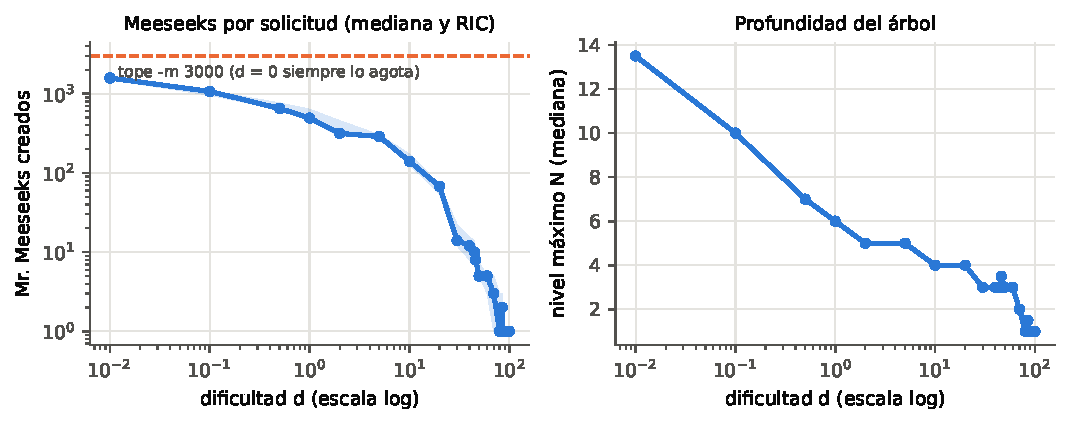
\includegraphics[width=\linewidth]{figs/e1_costo.pdf}
\caption{E1: Meeseeks creados y profundidad del árbol frente a la dificultad (ejes
logarítmicos en $d$; las solicitudes con $d=0$ no aparecen porque $\log 0$ no existe y
siempre llegan al tope).}
\label{fig:e1}
\end{figure}

\paragraph{Observaciones.}
\begin{itemize}[leftmargin=1.5em]
\item Para $d>85$ siempre basta un Meeseeks y $\Tt$ es prácticamente la duración
  simulada: el sistema operativo agrega menos de 1~ms.
\item Entre 45 y 85 se crean pocos Meeseeks (entre 1 y 13) gracias al Tiro Meeseeks y a
  que con 2 ayudantes la dificultad sube rápido. Se nota la discontinuidad del enunciado en
  $d=45$: con $d=46$ se piden 2 ayudantes y con $d=45$ se piden 5. Con 5 ayudantes se crean
  algo más de procesos (10 contra 8 en mediana), pero el árbol es menos profundo (3 contra
  4 niveles) y la tarea termina antes (0.213~s contra 0.333~s). Más paralelismo cambia
  procesos por tiempo.
\item Por debajo de $d\approx20$ el costo crece rápidamente: 68 Meeseeks con $d=20$, 288
  con $d=5$ y más de 1500 con $d=0.01$. Sin embargo, como la dilución multiplica la facilidad
  por casi 2.1 en cada generación, la profundidad solo crece como $\log(1/d)$: de 4 niveles
  con $d=10$ a 14 con $d=0.01$. El tiempo total sigue esa misma ley logarítmica.
\item Todas las tareas con $d>0$ se resolvieron (100\,\%). Todas las de $d=0$ terminaron
  en el tope de 3000 Meeseeks, con una mediana de 20 niveles, sin colapsar el sistema.
\end{itemize}

\begin{figure}[H]
\centering
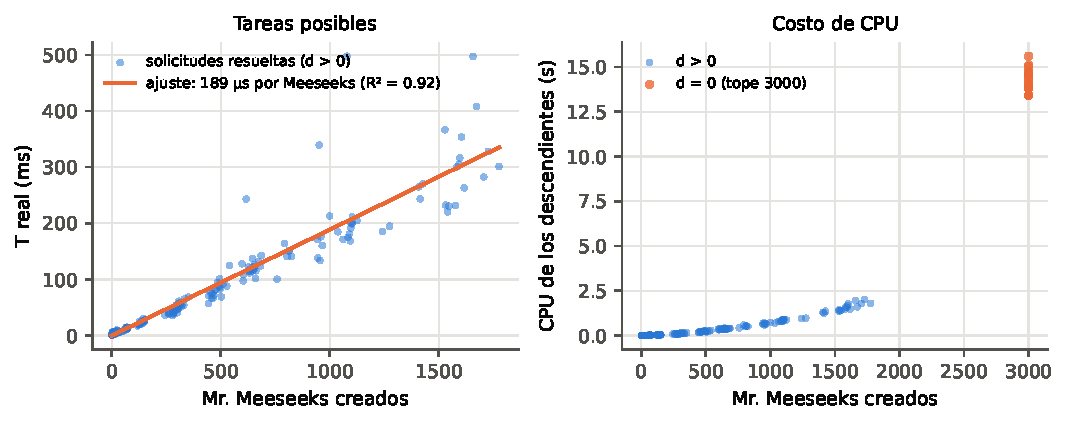
\includegraphics[width=\linewidth]{figs/e1_overhead.pdf}
\caption{E1: tiempo real (sin esperas simuladas) y CPU frente a la cantidad de Meeseeks
creados.}
\label{fig:e1b}
\end{figure}

\paragraph{Costo por Meeseeks.} En las solicitudes resueltas, el tiempo real crece de forma
lineal con la cantidad de Meeseeks: el ajuste da unos \EfitUs~µs de tiempo de pared por
Meeseeks ($R^2=\EfitR$) y unos \EfitCpuUs~µs de CPU. La CPU supera al tiempo de pared
porque hay dos núcleos trabajando en paralelo y porque cada \texttt{fork()} copia las tablas
de páginas del padre. En cambio, las tareas imposibles se salen de la recta (puntos naranja):
3000 Meeseeks consumen alrededor de 14~s de CPU, unas cinco veces lo que predice el
ajuste. La causa se analiza en E4.

\subsection{E2: duración aleatoria frente a duración fija}

Para tres dificultades se comparó la duración aleatoria uniforme en $[0.5, 5]$~s contra
una duración fija igual a su media (2.75~s), con 10 repeticiones cada una.

\begin{table}[H]
\centering\small
\begin{tabular}{rlrrrrr}
\toprule
$d$ & Duración & $T_{total}$ (s) & $T_{sim}$ (s) & $T_{real}$ (ms) & Meeseeks & Niv. \\
\midrule
90 & aleatoria 0.5-5 s & 2.90 $\pm$ 1.33 & 2.89 & 3.5 $\pm$ 1.4 & 1 & 1 \\
90 & fija 2.75 s & 2.75 $\pm$ 0.00 & 2.75 & 4.0 $\pm$ 1.5 & 1 & 1 \\
50 & aleatoria 0.5-5 s & 6.44 $\pm$ 2.00 & 6.43 & 8.2 $\pm$ 2.6 & 5 & 3 \\
50 & fija 2.75 s & 7.43 $\pm$ 1.74 & 7.42 & 9.7 $\pm$ 2.1 & 6 & 3 \\
20 & aleatoria 0.5-5 s & 5.53 $\pm$ 0.95 & 5.52 & 10.9 $\pm$ 3.5 & 28 & 4 \\
20 & fija 2.75 s & 8.43 $\pm$ 1.40 & 8.42 & 18.2 $\pm$ 5.6 & 63 & 4 \\
\bottomrule
\end{tabular}

\caption{E2: media $\pm$ desviación estándar; Meeseeks y niveles en mediana.}
\end{table}

\begin{figure}[H]
\centering
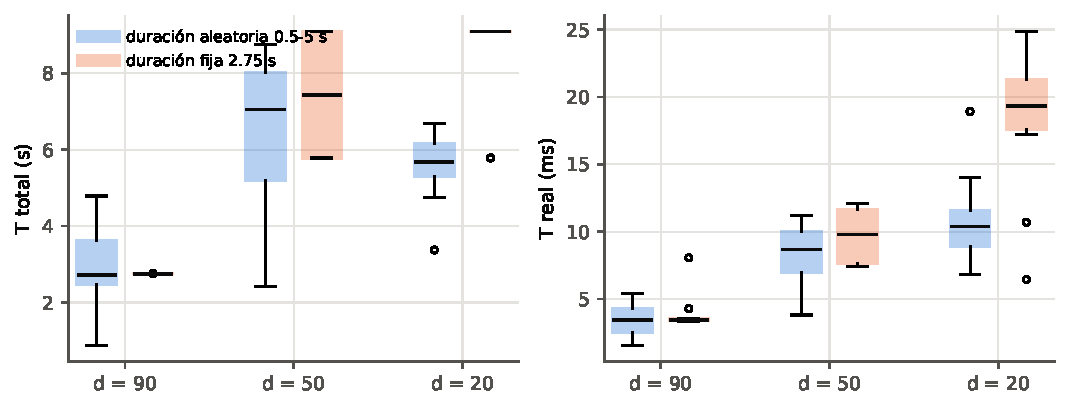
\includegraphics[width=\linewidth]{figs/e2_aleatorio.pdf}
\caption{E2: tiempo total y tiempo real según el tipo de duración.}
\end{figure}

\paragraph{Observaciones.}
\begin{itemize}[leftmargin=1.5em]
\item El tiempo total está dominado por completo por la espera simulada: $\Tt$ y $\Ts$
  difieren en milisegundos. Esto confirma que, para comparar el costo del sistema, hay que
  mirar $\Tr$ y no $\Tt$.
\item Con un solo Meeseeks ($d=90$) la media es la misma con ambas duraciones (2.90 contra
  2.75~s), como se espera, pero la aleatoria tiene una dispersión grande.
\item Con muchos Meeseeks ($d=20$) ocurre algo menos obvio: la duración aleatoria es
  \emph{más rápida} (5.53 contra 8.43~s) y crea menos de la mitad de los procesos (28 contra
  63). Cuando varias ramas trabajan en paralelo, la solución llega por la rama que
  terminó primero, y el mínimo de varias duraciones aleatorias es mucho menor que su media.
  Además, al resolverse antes, no alcanzan a nacer las generaciones siguientes. En la
  serie, un Meeseeks con suerte puede ahorrarle trabajo a todos los demás.
\item El tiempo real de un solo Meeseeks es de unos 3.5~ms tras dormir 2.75~s, mientras que
  en E1, tras dormir 0.1~s, era de 0.8~ms. La diferencia no viene del programa sino de la
  latencia para despertar: después de varios segundos de inactividad la máquina virtual
  pone a dormir los núcleos y reactivarlos cuesta algunos milisegundos.
\end{itemize}

\subsection{E3: comparación de los tres casos}

Se midió el tiempo real de cada tipo de solicitud que atiende un solo Meeseeks. Para el
caso A se usó $d=100$ con una duración de 1~µs, de modo que el tiempo medido sea
prácticamente solo el del mecanismo.

\begin{table}[H]
\centering\small
\begin{tabular}{lrrrrrr}
\toprule
Caso & n & Éxito & Media (ms) & Mediana (ms) & P95 (ms) & CPU (ms) \\
\midrule
A: texto d=100 (1 Meeseeks) & 200 & 100\,\% & 0.319 & 0.276 & 0.531 & 0.230 \\
B: calc (válido) & 150 & 100\,\% & 0.282 & 0.256 & 0.376 & 0.278 \\
B: calc (error) & 50 & 0\,\% & 0.253 & 0.230 & 0.407 & 0.254 \\
C: run true & 200 & 100\,\% & 2.400 & 2.332 & 2.851 & 2.253 \\
C: run false & 50 & 0\,\% & 2.133 & 2.019 & 2.721 & 2.135 \\
C: run ls /usr/bin & 50 & 100\,\% & 5.878 & 5.472 & 7.382 & 5.616 \\
C: run sleep 0.25 & 20 & 100\,\% & 255.429 & 255.288 & 256.103 & 4.929 \\
\bottomrule
\end{tabular}

\caption{E3: tiempo real por tipo de solicitud.}
\end{table}

\begin{figure}[H]
\centering
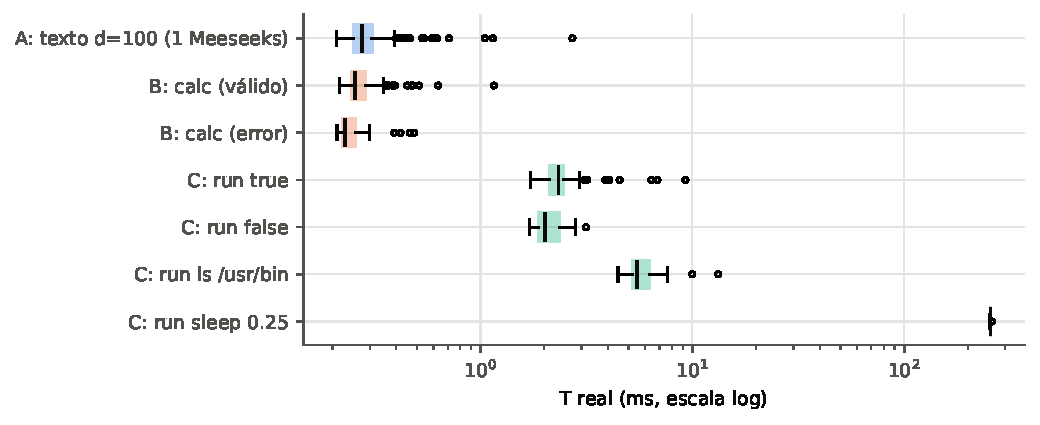
\includegraphics[width=\linewidth]{figs/e3_casos.pdf}
\caption{E3: distribución del tiempo real por caso (escala logarítmica).}
\end{figure}

\paragraph{Observaciones.}
\begin{itemize}[leftmargin=1.5em]
\item Los casos A (un Meeseeks) y B cuestan lo mismo, alrededor de 0.25 a 0.3~ms: ese es el
  costo base de crear un proceso con \texttt{fork()}, mandarle un mensaje por pipe, recibir
  la respuesta y recogerlo con \texttt{waitpid()}. Evaluar la expresión es despreciable
  frente a eso, y que la expresión tenga un error no cambia el tiempo.
\item El caso C es unas 9 veces más caro (unos 2.3~ms con \texttt{true}) porque el
  Meeseeks hace un segundo \texttt{fork()} y un \texttt{exec()} de \texttt{/bin/sh}, que a
  su vez carga y ejecuta el programa: cargar un ejecutable nuevo (abrir el archivo, mapear
  sus segmentos, enlazar bibliotecas dinámicas) cuesta mucho más que duplicar un proceso
  que ya está en memoria.
\item El resultado del programa externo no cambia el costo (\texttt{true} y \texttt{false}
  tardan lo mismo); lo que cambia es el trabajo del programa (\texttt{ls /usr/bin} tarda
  más del doble) y, sobre todo, si el programa espera: con \texttt{sleep 0.25} el tiempo
  real es de 255~ms, pero la CPU es de solo 5~ms. En el caso C no hay espera simulada, así
  que el tiempo del programa externo es tiempo real de la solicitud.
\end{itemize}

\subsection{E4: plan de contingencia}

\paragraph{E4a: semáforo de \emph{slots}.} Con $d=10$ y duración 0.1~s (15 repeticiones)
se varió la cantidad de Meeseeks que pueden trabajar a la vez.

\begin{table}[H]
\centering\small
\begin{tabular}{rrrrrrr}
\toprule
Slots (\texttt{-a}) & $T_{total}$ (s) & $T_{real}$ (ms) & Meeseeks & Pico vivos & Niv. & CPU (ms) \\
\midrule
2 & 0.605 & 5.0 & 9 & 9 & 5 & 10.0 \\
4 & 0.465 & 4.8 & 16 & 14 & 5 & 11.4 \\
8 & 0.467 & 6.7 & 28 & 24 & 5 & 16.1 \\
16 & 0.468 & 9.3 & 44 & 38 & 5 & 23.6 \\
32 & 0.343 & 12.9 & 66 & 59 & 4 & 24.9 \\
64 & 0.350 & 20.0 & 100 & 92 & 4 & 37.6 \\
128 & 0.353 & 22.7 & 142 & 133 & 4 & 44.3 \\
512 & 0.352 & 22.1 & 140 & 135 & 4 & 42.3 \\
\bottomrule
\end{tabular}

\caption{E4a: medianas según la cantidad de \emph{slots}.}
\end{table}

\begin{figure}[H]
\centering
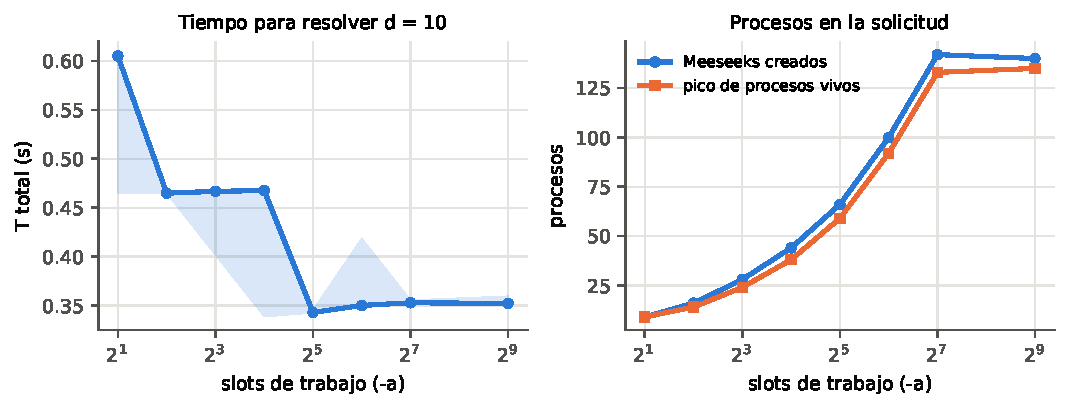
\includegraphics[width=\linewidth]{figs/e4a_slots.pdf}
\caption{E4a: efecto del semáforo de \emph{slots} con $d=10$.}
\end{figure}

Restringir los \emph{slots} reduce mucho los procesos creados (de 142 a 9) y la CPU (de
44 a 10~ms) a cambio de un poco más de tiempo (de 0.35 a 0.61~s). Con pocos \emph{slots}
el árbol crece en profundidad en lugar de en anchura: los primeros Meeseeks en conseguir
\emph{slot} siguen diluyendo la tarea hacia abajo, y cuando uno la resuelve todavía no han
nacido muchos de sus primos. Con muchos \emph{slots} se crean procesos que al final no
sirven. Por encima de 128 no hay diferencia porque el árbol nunca necesita más.

\paragraph{E4b: tope total con tareas imposibles.} Con $d=0$ y duración 0.1~s (5
repeticiones) se varió el tope \texttt{-m}.

\begin{table}[H]
\centering\small
\begin{tabular}{rrrrrrrr}
\toprule
Tope (\texttt{-m}) & Éxito & $T_{total}$ (s) & $T_{real}$ (s) & Meeseeks & Pico vivos & Niv. & CPU (s) \\
\midrule
100 & 0\,\% & 0.71 & 0.013 & 100 & 98 & 4 & 0.04 \\
250 & 0\,\% & 1.02 & 0.021 & 250 & 247 & 5 & 0.09 \\
500 & 0\,\% & 1.79 & 0.038 & 500 & 499 & 7 & 0.35 \\
1000 & 0\,\% & 3.89 & 0.040 & 1000 & 999 & 11 & 1.56 \\
2000 & 0\,\% & 8.57 & 0.071 & 2000 & 1999 & 17 & 6.01 \\
3000 & 0\,\% & 13.27 & 1.818 & 3000 & 2994 & 20 & 14.07 \\
5000 & 0\,\% & 29.52 & 14.569 & 5000 & 4951 & 23 & 44.30 \\
\bottomrule
\end{tabular}

\caption{E4b: medianas según el tope de Meeseeks para una tarea imposible.}
\end{table}

\begin{figure}[H]
\centering
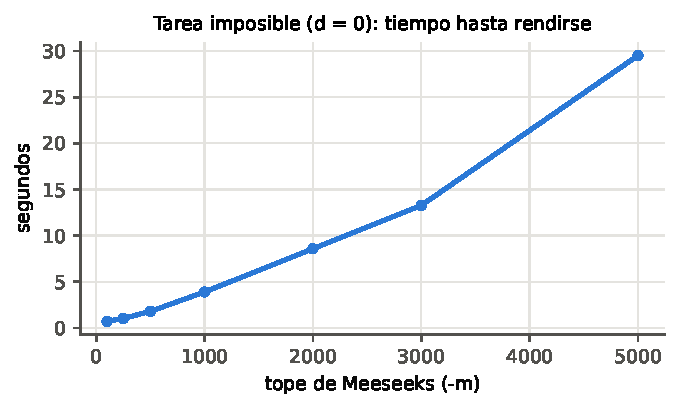
\includegraphics[width=0.62\linewidth]{figs/e4b_tope.pdf}
\caption{E4b: tiempo hasta rendirse frente al tope.}
\end{figure}

El tope cumple su función: ninguna tarea imposible pasó del límite y todas terminaron en
segundos. Sin embargo, el costo no es lineal en el tope. Al duplicar de 1000 a 2000
Meeseeks la CPU se multiplica por casi 4, y con 5000 el programa usó unos 44~s de CPU en
30~s de pared, es decir, los dos núcleos casi saturados. El pico de procesos vivos es
prácticamente igual al tope, porque en una tarea imposible casi nadie termina hasta que se
rinde todo el árbol.

La causa es una decisión de diseño. Un padre que quiere crear un ayudante y no encuentra
\emph{slot} no se bloquea en \texttt{sem\_wait}, porque necesita seguir atendiendo su pipe
(podría llegarle \texttt{M\_STOP}); en su lugar vuelve a intentarlo cada 25~ms con
\texttt{poll()}. Con miles de padres en esa situación, el sistema hace miles de intentos por
segundo y la cantidad de intentos crece con la cantidad de padres multiplicada por el tiempo
que esperan, lo que da un costo cuadrático. Es una forma de espera activa. Una mejora sería
que los Meeseeks que liberan un \emph{slot} despierten a los que esperan por un descriptor
(por ejemplo un pipe de fichas o un \texttt{eventfd}) que se pueda vigilar con el mismo
\texttt{poll()}; así la espera sería pasiva sin dejar de atender el pipe.

\subsection{E5: sensibilidad a la ganancia de dilución}

La ganancia $g$ controla qué tan rápido se simplifica la tarea entre generaciones. Se
probaron tres valores con tres dificultades (20 repeticiones, duración 0.1~s).

\begin{table}[H]
\centering\small
\begin{tabular}{rrrrrrrr}
\toprule
$d$ & $g$ & Éxito & Meeseeks (med.) & Máx. & Niv. & $T_{total}$ (s) & $T_{real}$ (ms) \\
\midrule
50 & 0.25 & 100\,\% & 11 & 29 & 4 & 0.333 & 3.1 \\
50 & 0.5 & 100\,\% & 5 & 13 & 3 & 0.212 & 2.3 \\
50 & 1 & 100\,\% & 5 & 7 & 3 & 0.212 & 2.0 \\
20 & 0.25 & 100\,\% & 136 & 268 & 4 & 0.351 & 21.0 \\
20 & 0.5 & 100\,\% & 65 & 77 & 4 & 0.340 & 10.4 \\
20 & 1 & 100\,\% & 14 & 24 & 3 & 0.213 & 3.1 \\
5 & 0.25 & 100\,\% & 488 & 635 & 6 & 0.676 & 76.1 \\
5 & 0.5 & 100\,\% & 285 & 371 & 5 & 0.504 & 44.0 \\
5 & 1 & 100\,\% & 114 & 135 & 4 & 0.348 & 17.3 \\
\bottomrule
\end{tabular}

\caption{E5: efecto de la ganancia $g$ (medianas).}
\end{table}

\begin{figure}[H]
\centering
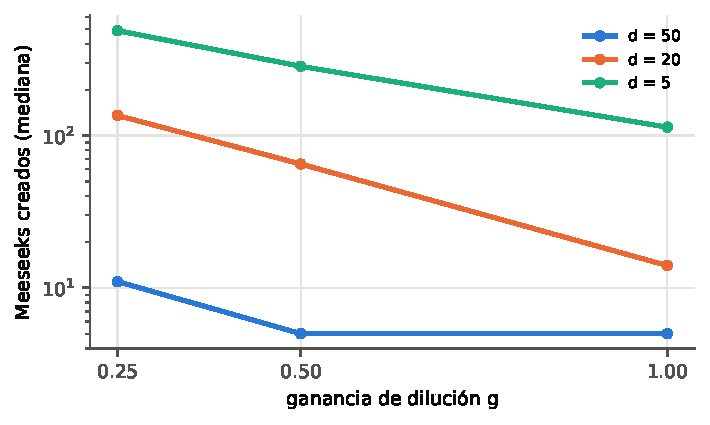
\includegraphics[width=0.66\linewidth]{figs/e5_ganancia.pdf}
\caption{E5: Meeseeks creados según la ganancia.}
\end{figure}

Con $g=1$ la dilución es tan rápida que incluso $d=5$ se resuelve con alrededor de 110
Meeseeks y 4 niveles; con $g=0.25$ se necesitan unos 490 y 6 niveles. El efecto es mayor para las
dificultades medianas ($d=20$: de 136 a 14 Meeseeks, casi diez veces menos) que para las
fáciles. El valor por defecto $g=0.5$ es un término medio: deja ver árboles grandes para
tareas difíciles, como en la serie, sin que las tareas medianas generen cientos de
procesos.

\subsection{E6: tareas que superan el tiempo máximo}\label{sec:e6}

El enunciado pregunta qué pasa si una solicitud muy difícil no se cumple en el tiempo
máximo y cuánto tiempo adicional se necesita. Para responderlo se usó el modo
experimento (\texttt{-x}): al vencer el plazo la Box anuncia el caos pero no termina los
procesos, y se mide cuándo llega la solución. Para poder repetir cada caso se trabajó a
escala: tiempo máximo de 30~s, 16 \emph{slots}, duración fija de 0.25~s y tope de 30\,000
Meeseeks. Se hicieron 3 corridas por dificultad, desde $d=1$ hasta $d=10^{-9}$.

\begin{table}[H]
\centering\small
\begin{tabular}{rrrrrrrr}
\toprule
$d$ & Resuelta & $T_{total}$ (s) & Extra sobre 30 s & Meeseeks & Niv. & Pico vivos & CPU (s) \\
\midrule
1 & sí & 1.9 & 0.0 & 92 & 7 & 80 & 0.07 \\
1 & sí & 2.3 & 0.0 & 101 & 8 & 89 & 0.11 \\
1 & sí & 2.3 & 0.0 & 101 & 8 & 92 & 0.10 \\
0.01 & sí & 4.7 & 0.0 & 184 & 13 & 180 & 0.40 \\
0.01 & sí & 5.8 & 0.0 & 233 & 15 & 203 & 0.53 \\
0.01 & sí & 4.7 & 0.0 & 186 & 13 & 181 & 0.38 \\
0.0001 & sí & 9.1 & 0.0 & 335 & 20 & 299 & 1.21 \\
0.0001 & sí & 8.4 & 0.0 & 322 & 19 & 284 & 1.16 \\
0.0001 & sí & 9.6 & 0.0 & 337 & 20 & 313 & 1.44 \\
1e-06 & sí & 13.9 & 0.0 & 443 & 25 & 428 & 2.72 \\
1e-06 & sí & 13.0 & 0.0 & 436 & 25 & 391 & 2.43 \\
1e-06 & sí & 14.7 & 0.0 & 476 & 26 & 448 & 3.02 \\
1e-09 & sí & 24.0 & 0.0 & 687 & 35 & 646 & 6.79 \\
1e-09 & sí & 24.9 & 0.0 & 724 & 34 & 666 & 6.86 \\
1e-09 & sí & 351.0 & 321.0 & 5059 & 34 & 4543 & 579.12 \\
\bottomrule
\end{tabular}

\caption{E6: cada corrida con \texttt{-T 30 -x -a 16}. ``Extra'' es el tiempo que pasó
después de decretado el caos hasta que llegó la solución.}
\end{table}

\begin{figure}[H]
\centering
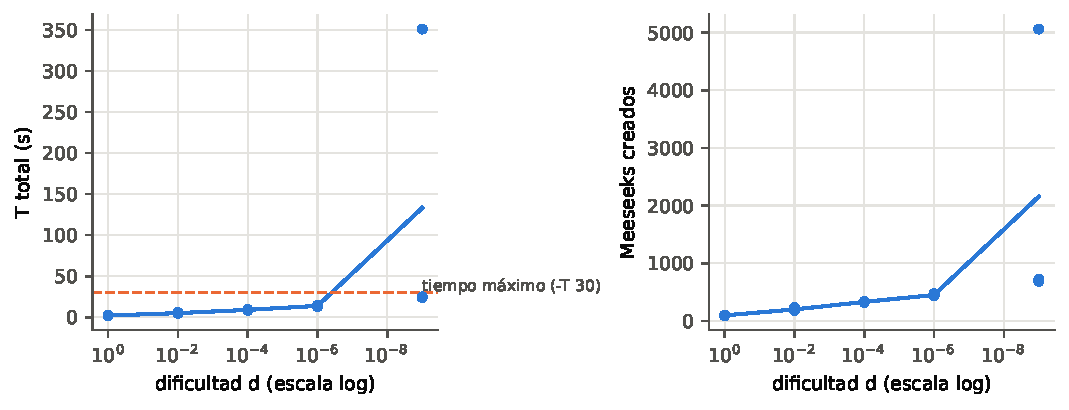
\includegraphics[width=\linewidth]{figs/e6_extra.pdf}
\caption{E6: tiempo total y Meeseeks creados para dificultades muy pequeñas.}
\end{figure}

\paragraph{Observaciones.}
\begin{itemize}[leftmargin=1.5em]
\item Mientras el sistema no se sature, el costo crece de forma logarítmica: cada factor de
  100 en la dificultad agrega unos 5 niveles y unos 4 a 5~s. Incluso $d=10^{-9}$ se resolvió
  en dos de tres corridas en unos 24~s, por debajo del máximo, con unos 700 Meeseeks.
\item La tercera corrida con $d=10^{-9}$ es el caso que pide el enunciado: superó los 30~s,
  se decretó el caos y, sin terminar el programa, la solución llegó a los 351~s, es decir,
  \textbf{321~s adicionales}. Lo notable es que la espera simulada del camino ganador fue de
  solo 22.5~s: casi todo el tiempo (328~s) fue tiempo real del sistema. Se crearon 5059
  Meeseeks, con 4543 vivos a la vez, que consumieron 579~s de CPU en dos núcleos.
\item La explicación es la misma que en E4b. Por azar, ese árbol creció más ancho que los
  otros; con miles de padres esperando un \emph{slot} y reintentando cada 25~ms, la CPU se
  satura en espera activa, los Meeseeks que sí trabajan se planifican tarde y el árbol
  avanza cada vez más lento, lo que a su vez deja más padres esperando. Es una
  retroalimentación positiva: pasado cierto tamaño, la tarea no se vuelve un poco más lenta,
  sino un orden de magnitud más lenta.
\item Conclusión de la prueba: el tiempo adicional que necesita una tarea muy difícil no es
  predecible a partir de su dificultad, porque depende de si el árbol cruza el umbral de
  saturación. Por debajo del umbral bastan segundos; por encima, varios minutos. Esto
  justifica que el tiempo máximo exista y que su acción sea terminar todo el grupo de
  procesos: seguir esperando puede costar mucho más que reintentar la solicitud.
\end{itemize}

A escala real (300~s de máximo y duraciones de 0.5 a 5~s) cada generación tarda en promedio
2.75~s en lugar de 0.25~s, por lo que el mismo árbol necesitaría unas 11 veces más tiempo
simulado: una tarea con $d=10^{-9}$ (unos 34 niveles) pasaría de los 300~s solo por las
esperas, aun sin saturación. Por esa razón la prueba se hizo a escala y no con los 5
minutos completos, que habrían requerido horas por corrida. La terminación por caos con un
tiempo máximo real se muestra en la corrida de la sección~\ref{sec:corridas}.


% ===========================================================================
\section{Conclusiones}

\begin{itemize}[leftmargin=1.5em]
\item Se implementó en un único programa en C la Box de Mr.\ Meeseeks con los tres tipos de
  solicitud. Todos los procesos ejecutan el mismo código, se crean con \texttt{fork()}, se
  comunican solo por pipes y comparten contadores protegidos por semáforos POSIX en memoria
  compartida.
\item La Ley de Dilución logística, con $d=0$ como punto fijo, cumple a la vez dos
  requisitos que parecen opuestos: cualquier tarea posible termina resolviéndose y una
  imposible jamás. Los experimentos muestran que la profundidad crece como $\log(1/d)$ y que
  la cantidad de Meeseeks crece muy rápido al acercarse a 0, como en la serie.
\item La concurrencia trajo problemas reales, no solo teóricos. Varios Meeseeks podían
  resolver la tarea a la vez (se corrigió con una victoria exclusiva en sección crítica) y el
  semáforo de \emph{slots} produjo un interbloqueo que cumplía las cuatro condiciones de
  Coffman (se corrigió liberando el \emph{slot} al pasar a esperar). Ninguno de los dos se
  habría notado sin probar con tareas difíciles.
\item Crear un Meeseeks cuesta unos 0.25~ms y algo menos de 0.2~ms adicionales por cada uno
  en un árbol grande; ejecutar un programa externo cuesta unas 9 veces más por el
  \texttt{exec}. En todas las solicitudes, el tiempo total lo domina la espera simulada,
  por eso el tiempo real debe medirse restando la espera del camino crítico y no la suma de
  todas las esperas.
\item Cuando hay paralelismo, la aleatoriedad ayuda: con duración aleatoria la tarea se
  resolvió antes y con menos procesos, porque gana la rama más rápida.
\item El plan de contingencia funcionó en todas las pruebas: ninguna tarea imposible colapsó
  el sistema. Aun así, la espera por \emph{slots} con sondeo periódico crece en forma
  cuadrática y llega a saturar la CPU con miles de procesos; una espera pasiva sería la
  siguiente mejora.
\item El tiempo máximo no es solo una protección contra tareas imposibles. Las tareas muy
  difíciles pero posibles también pueden superarlo, y entonces terminar el programa
  significa perder una solución que estaba en camino (sección~\ref{sec:e6}). Por eso el
  tiempo máximo es una decisión sobre cuánto se está dispuesto a esperar, y su valor debe
  considerar la profundidad que puede alcanzar el árbol.
\end{itemize}

% ===========================================================================
\begin{thebibliography}{9}
\bibitem{silberschatz} A.~Silberschatz, P.~B.~Galvin y G.~Gagne, \emph{Operating System
  Concepts}, 10.ª ed. Hoboken, NJ, EE.~UU.: Wiley, 2018. Caps.~3 (procesos), 6 y 7
  (sincronización) y 8 (interbloqueos).
\bibitem{blp} N.~Matthew y R.~Stones, \emph{Beginning Linux Programming}, 4.ª ed.
  Indianápolis, IN, EE.~UU.: Wiley, 2008. Caps.~11 (procesos y señales), 13 (comunicación
  entre procesos: pipes) y 14 (semáforos, memoria compartida y colas de mensajes).
\bibitem{kerrisk} M.~Kerrisk, \emph{The Linux Programming Interface}. San Francisco, CA,
  EE.~UU.: No Starch Press, 2010. Caps.~24 a 26 (\texttt{fork}, \texttt{exit},
  \texttt{wait}), 44 (pipes), 53 (semáforos POSIX) y 63 (\texttt{poll}).
\bibitem{coffman} E.~G.~Coffman, M.~Elphick y A.~Shoshani, ``System deadlocks'',
  \emph{ACM Computing Surveys}, vol.~3, n.º~2, pp.~67--78, 1971.
\bibitem{man} The Linux man-pages project, \texttt{fork(2)}, \texttt{pipe(7)},
  \texttt{sem\_overview(7)}, \texttt{poll(2)}, \texttt{prctl(2)}, \texttt{getrusage(2)}.
  [En línea]. Disponible: \url{https://man7.org/linux/man-pages/}
\bibitem{rm} J.~Roiland y D.~Harmon (creadores), ``Meeseeks and Destroy'', \emph{Rick and
  Morty}, temp.~1, ep.~5. Adult Swim, 2014.
\end{thebibliography}


\end{document}
